\documentclass[11pt]{article}
\usepackage{hyperref}
\usepackage{graphicx}

\title{P4 Submission}
\author{Nick Werle}
\date{\today}
\begin{document}
	\maketitle
	\section{Preamble}
	The code and other files, in addition to being included with the pilot submission as required, will be available at \url{https://github.com/NickWer/CEG3900_P4} on Thursday, March 16th.
	\section{Task 1}
	My program works well, with no bugs or crashes that I am aware of. To test, I made the file many times larger (copy and pasted the original 240k log until it was 300MB) and it still ran well. Additionally, using a script called memusg from \url{https://gist.github.com/netj/526585}\footnote{This script is included in my repository as a submodule.}, I was able to verify that the memory consumption of my implementation did not noticeably grow with the size of the input.
	
	I developed this program by creating a package for parsing, which will hopefully be trivial enough to modify for the later parts of the assignment. Using streams and regex it searches each line of the log against the regex string and extracts the IP address if possible. I think the callback that I put in place will be valuable for the later portions, and what code there is will be simple to modify.
	\section{Task 2}
	See figures 1-4 for the screenshots of this application running. Note that they may end up in funny places throughout the document, because that's what \LaTeX\ likes to do.
	
	My application works well enough. One thing that could be improved is that, when clicking either processes button, the calculation is run on the UI thread and so the application hangs while it processes the log.
	
	Building this application wasn't too terrible but also certainly came with many minor issues. Passing data between activities is surprisingly difficult if you actually want to do it the right way, and need to send more than a simple integer or string. I decided that this wasn't worth figuring out given my somewhat limited time and the simplicity of the application, so I just used a global static class to hold the Stream object I wanted to pass.
	
	\begin{figure}[ht]
		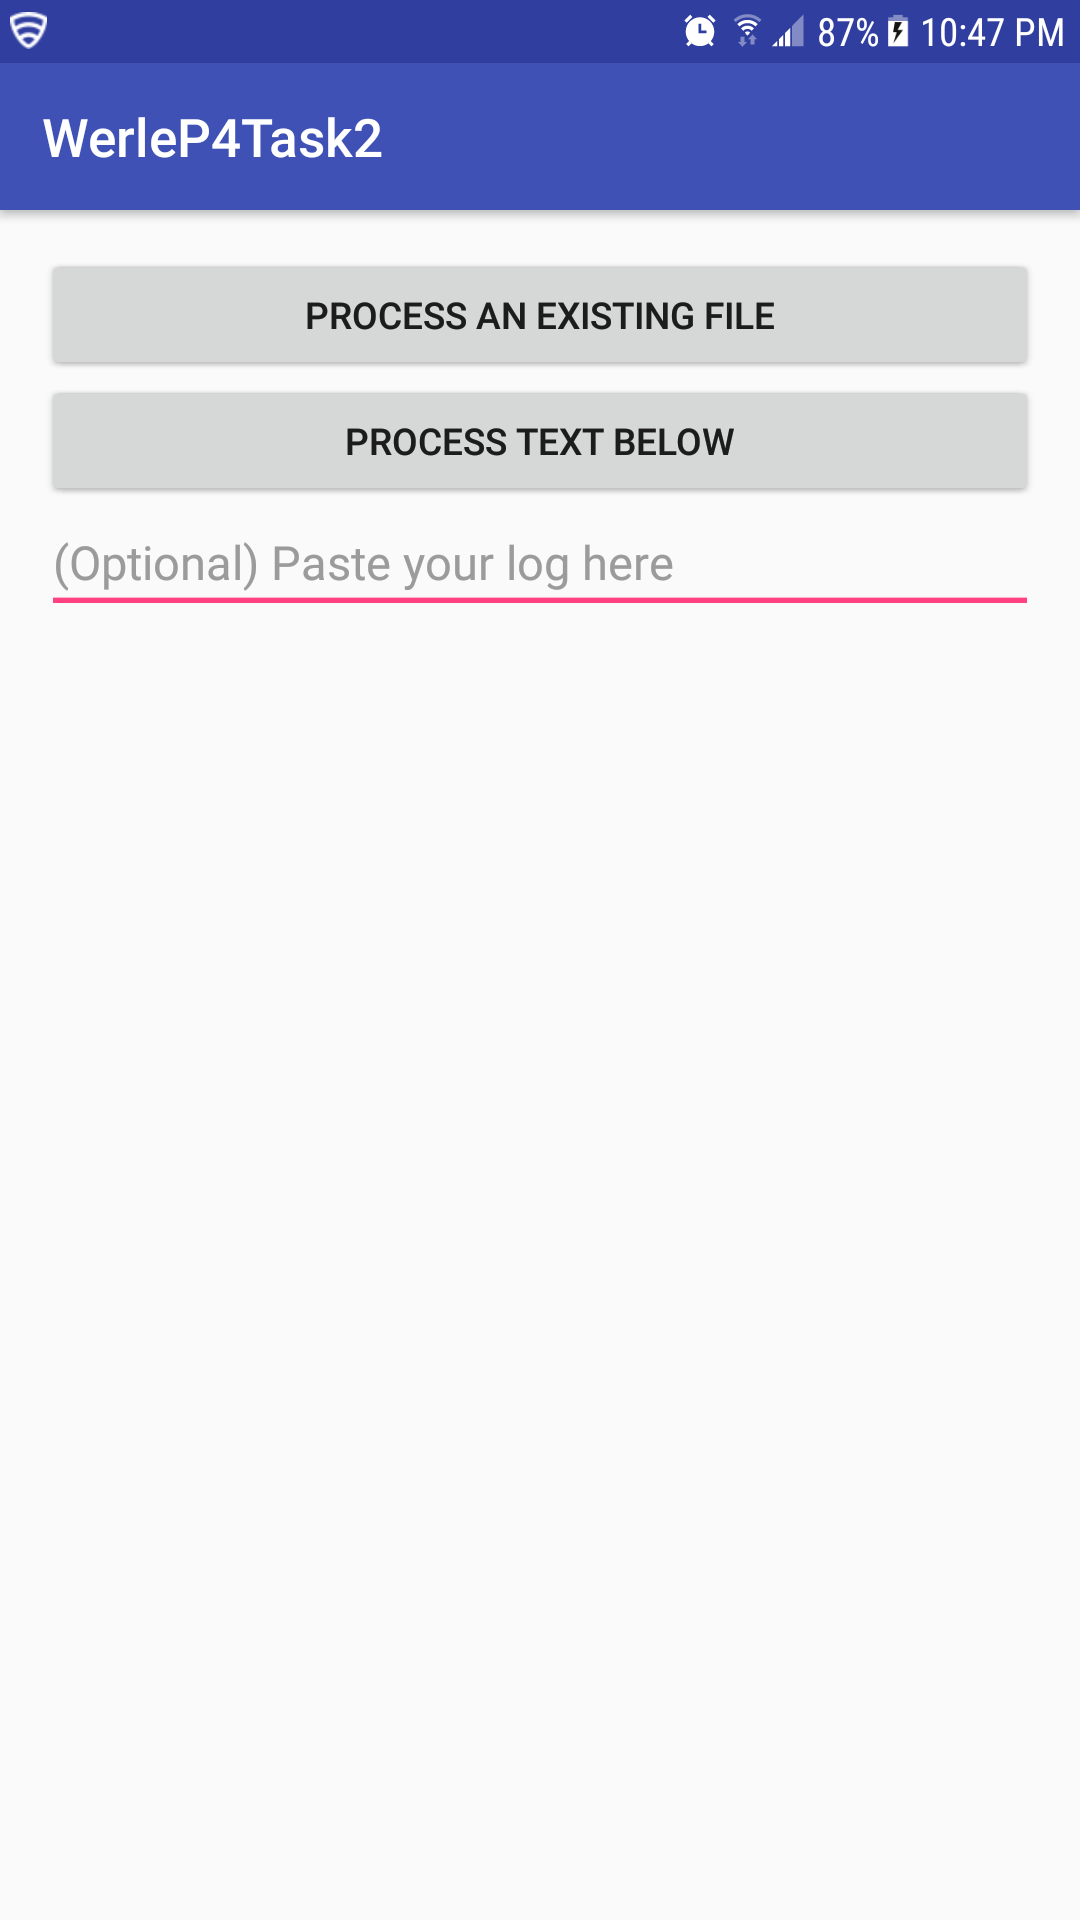
\includegraphics[width=3in]{img/t2s1.png}
		\centering
		\caption{Home screen}
	\end{figure}
	\begin{figure}[ht]
		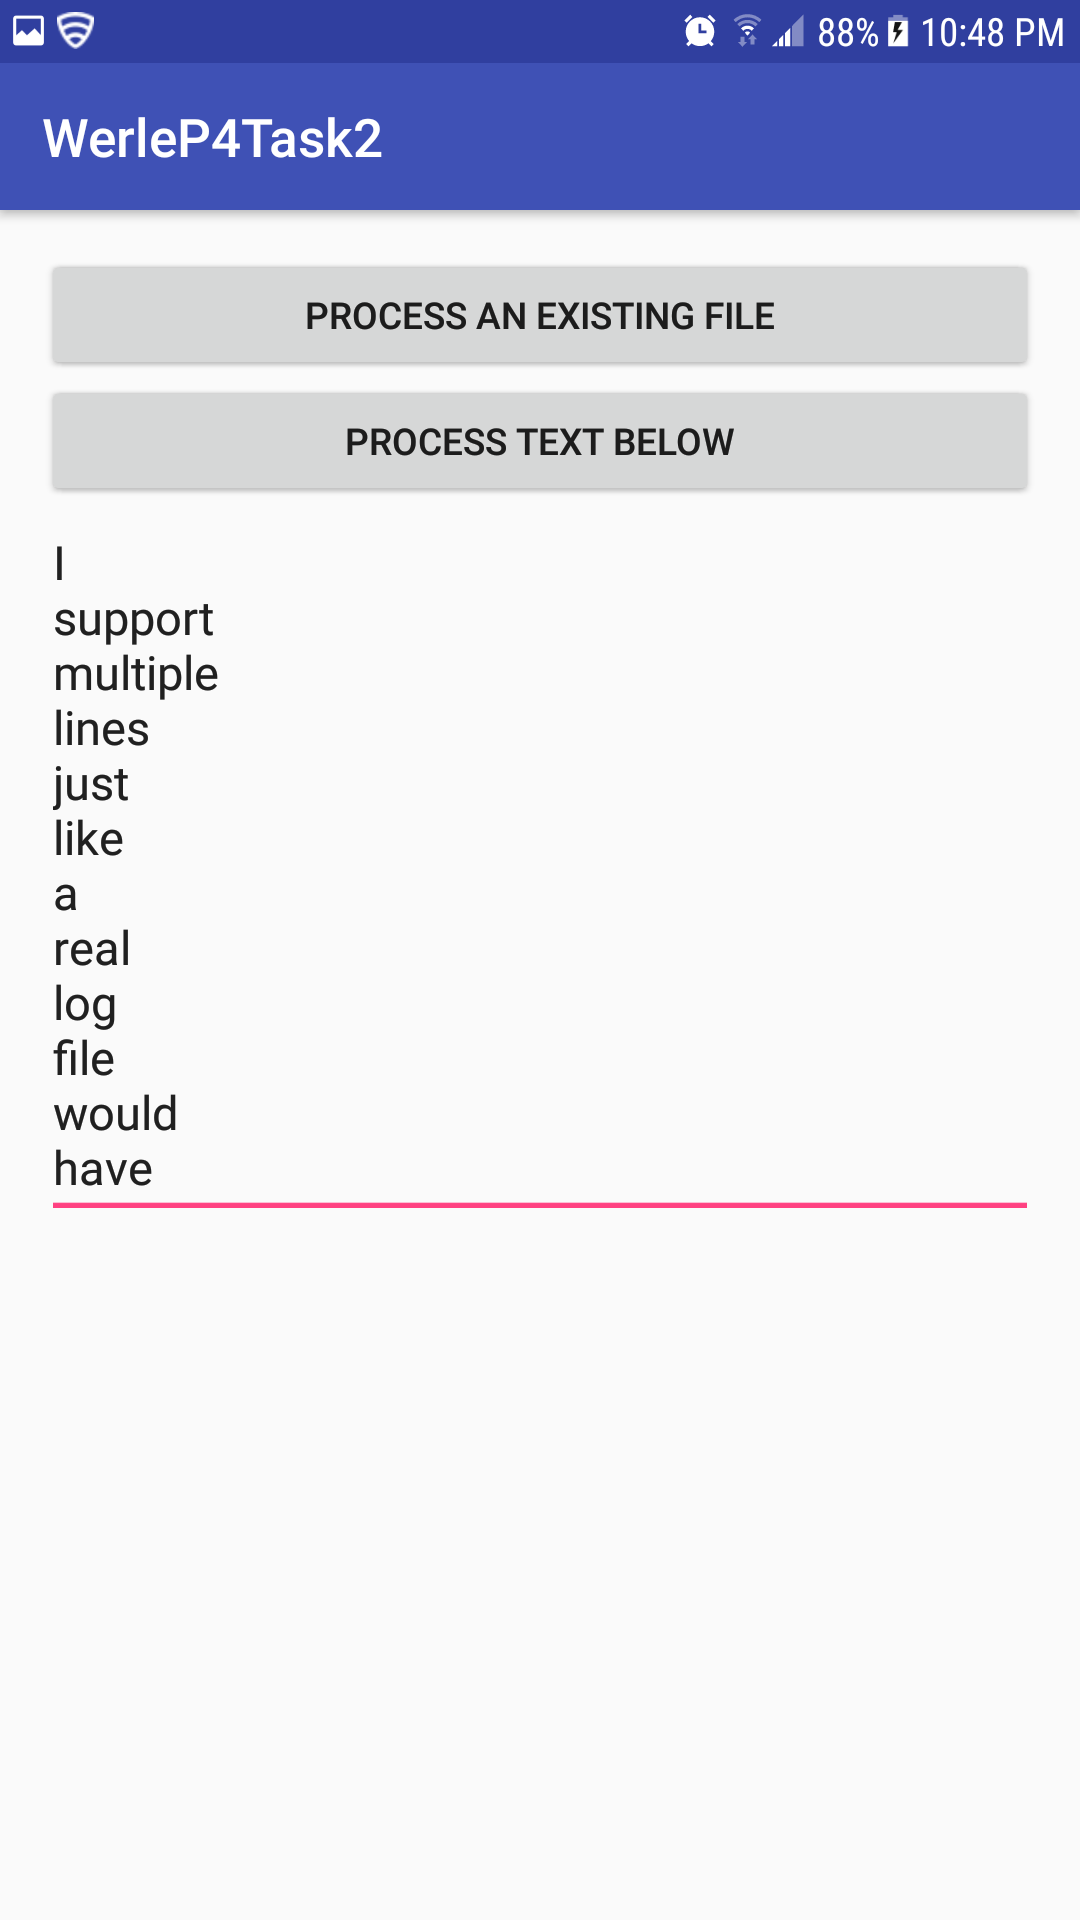
\includegraphics[width=3in]{img/t2s2.png}
		\centering
		\caption{Some text in the log textbox (It is multiline)}
	\end{figure}
	\begin{figure}[ht]
	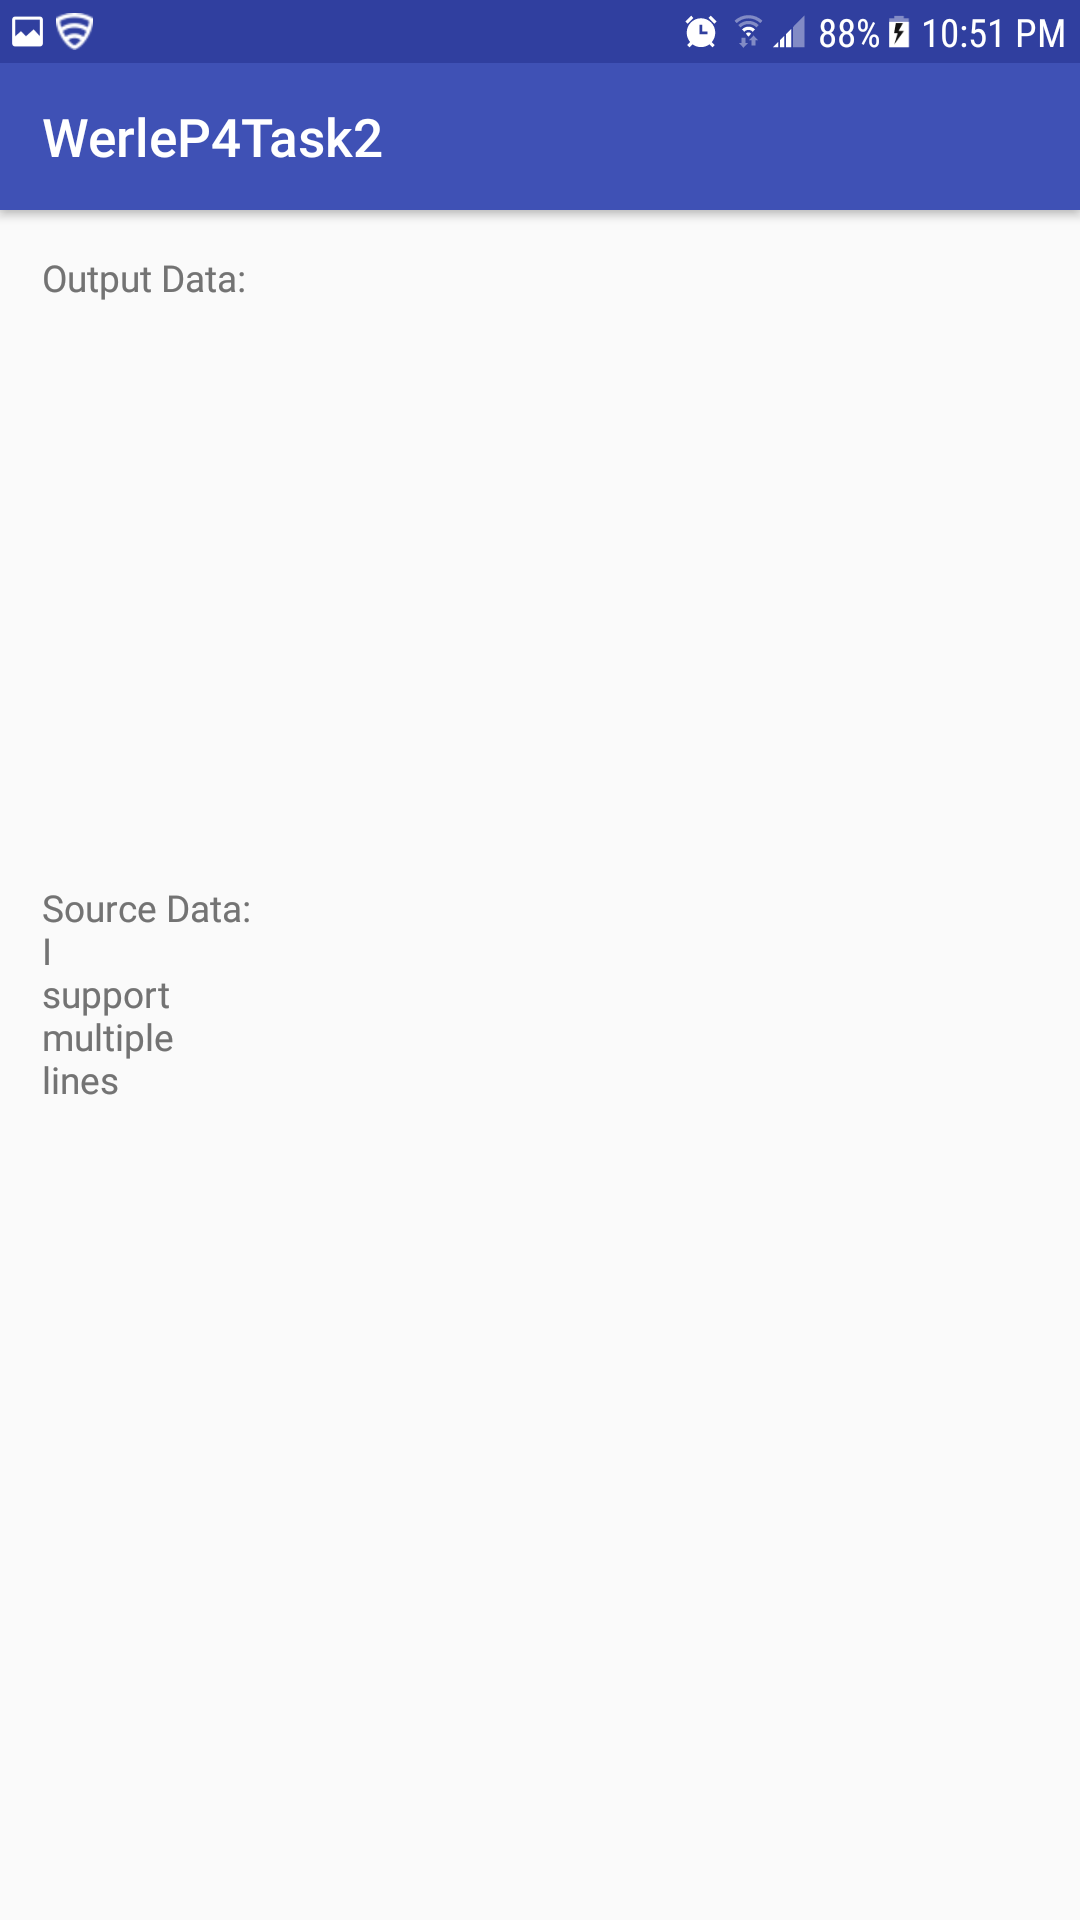
\includegraphics[width=3in]{img/t2s3.png}
	\centering
	\caption{Example output from a nonsense input}
	\end{figure}
	\begin{figure}[ht]
	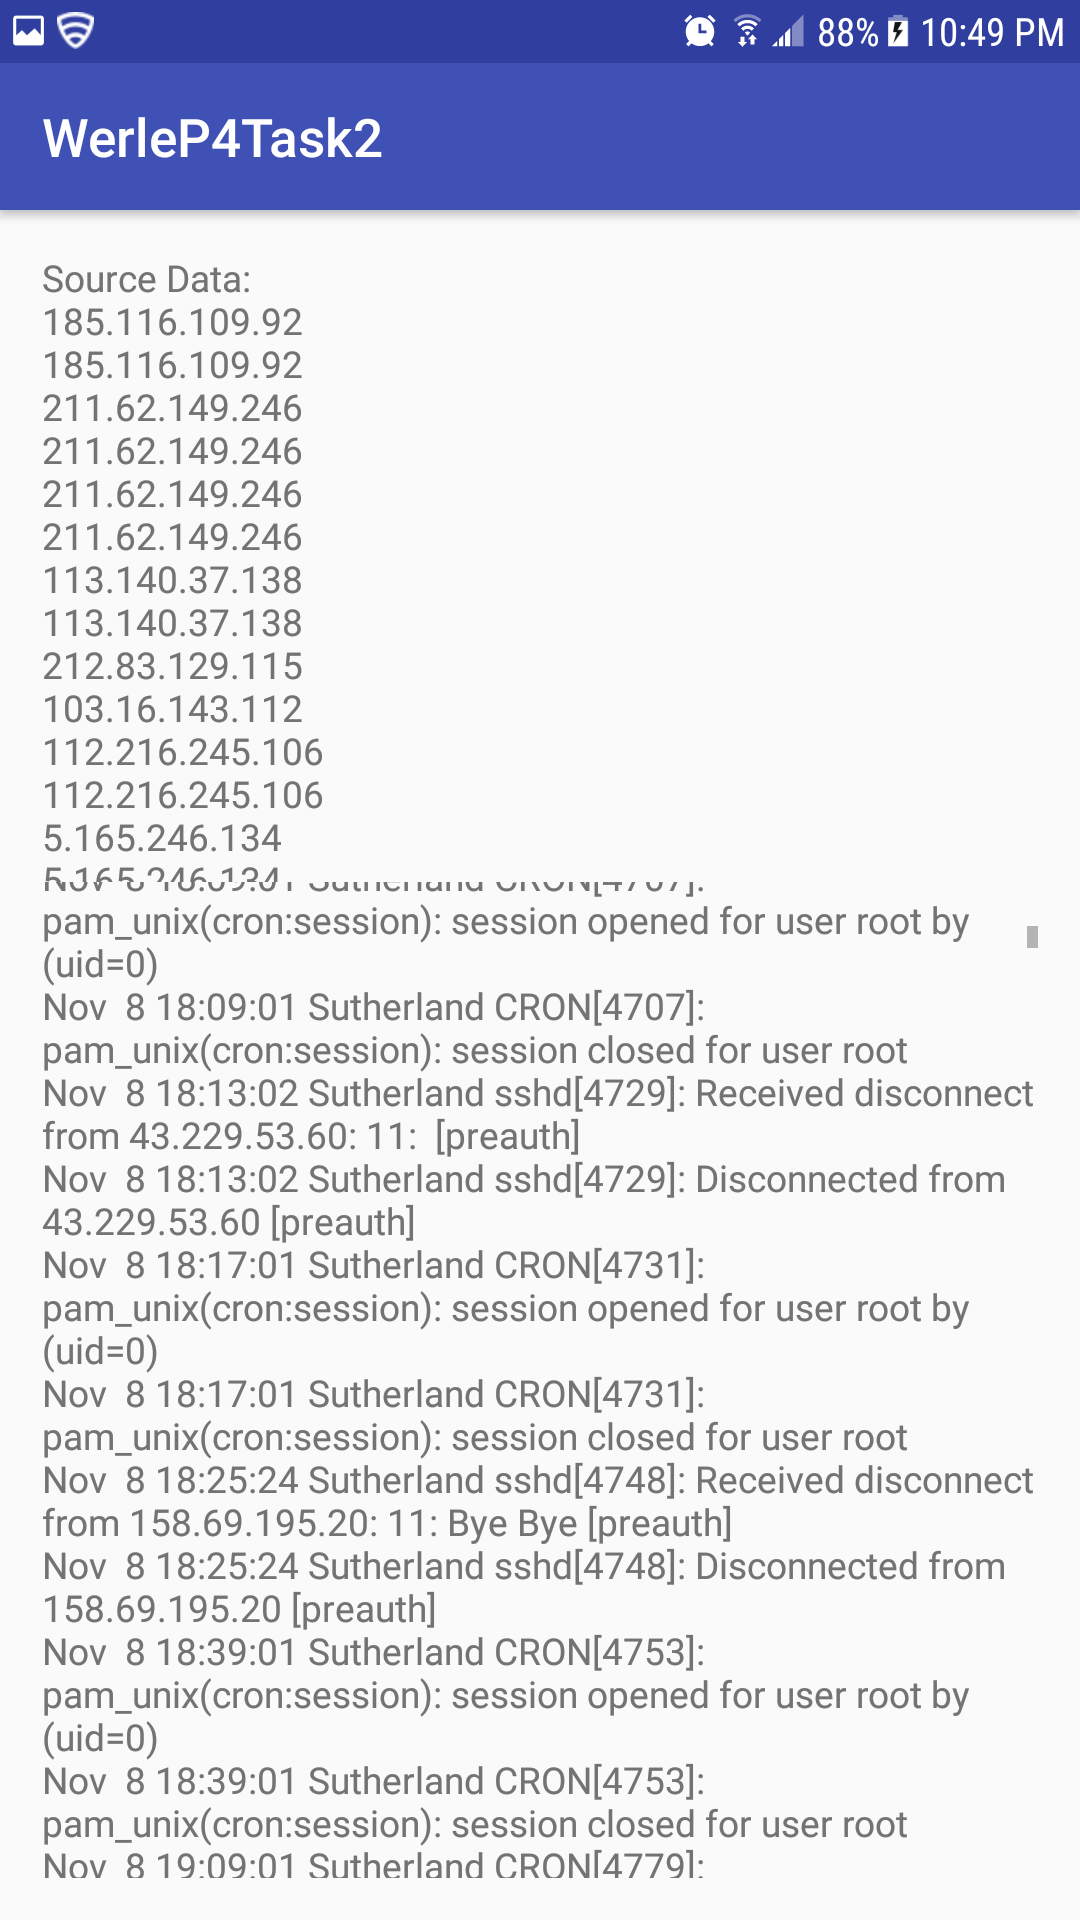
\includegraphics[width=3in]{img/t2s4.png}
	\centering
	\caption{Example output from the provided input. You can kind of see that the lower portion of text is scrollable (the scrollbar is visible), but it's hard to capture that in a screenshot.}
	\end{figure}
	\section{Task 3}
	The source for this program is available in the Task 3 folder. I used the following input to test my program:
\begin{verbatim}
https://www.gutenberg.org/files/38280/38280-0.txt
http://www.gutenberg.org/cache/epub/20/pg20.txt
http://www.gutenberg.org/cache/epub/8209/pg8209.txt
https://www.gutenberg.org/files/25340/25340-0.txt
https://www.gutenberg.org/files/25340/25340-0.txt
http://www.gutenberg.org/cache/epub/8388/pg8388.txt
http://www.gutenberg.org/cache/epub/22312/pg22312.txt
http://www.gutenberg.org/cache/epub/2939/pg2939.txt
http://www.gutenberg.org/cache/epub/36446/pg36446.txt
http://www.gutenberg.org/cache/epub/5891/pg5891.txt
\end{verbatim}
Which generates the following output (n = 10):
\begin{verbatim}
the - 57874
of - 31890
and - 29439
to - 19994
a - 16415
in - 16365
is - 9199
i - 8946
that - 8150
\end{verbatim}

My solution works well, as best I can tell. It does not attempt to strip out html or anything similar, and so it generally assumes that input is plaintext. Additionally it will only be compatible with the standard 26/52 character English alphabet. As I understand it this solution works with ASCII as well as other UTF encodings, though I have not tested this.

The experience of developing this was overall not very different from Task 1, though the optimization phase did strain my familiarity with the Java regex/Pattern API, and I've never used the reduction capabilities of streams either. Once again I took the approach of making a general enough solution that I will be able to re-purpose my package for the android application, however this time I took a more straightforward approach by returning the list and allowing the package user to manipulate it as they please.

One thing I found during development is that it is considerably faster to use regex to match the words themselves (my current solution), rather than their delimiters (my initial solution). While this arguable produces less true results (e.g. hyphenated words will not be treated thusly), it simplifies the sanitation process considerably (lowercasing, removing trailing punctuation, etc.) and avoids multiple, costly passes over the dataset as different map and filter operations are applied for sanitization. You could, of course, apply one very good map or filter that does the sanitation in a single step, but by grabbing the words directly, you can avoid even that single extra pass, speeding up the output considerably.

\section{Task 4}
\end{document}
